\documentclass[a4paper, 12pt]{article}

\usepackage[T2A]{fontenc}
\usepackage[utf8]{inputenc}
\usepackage[english,russian]{babel}
\usepackage[left=15mm, top=20mm, right=15mm, bottom=20mm, nohead, nofoot]{geometry}

\usepackage{graphicx}
\usepackage{wrapfig}
\usepackage{afterpage}
\usepackage{amsmath, amsfonts, amssymb, amsthm, mathtools}
\author{Хомутов Андрей, группа Б06-903}
\title{Лабораторная работа 3.2.2* \\ Резонанс токов
}
\date{21 сентября 2020 г.}

\begin{document}

\maketitle
\thispagestyle{empty}
\newpage

\section*{Цель работы} 
\begin{enumerate}
    \item Изучение параллельной цепи переменного тока
    \item Наблюдение резонанса токов
\end{enumerate}


\section*{В работе используются}
Лабораторный автотрансформатор (ЛАТР),
разделительный понижающий трансформатор, емкость, дроссель с пе-
ременной индуктивностью, три амперметра, вольтметр, реостат, элек-
тронный осциллограф, омметр, мост переменного тока. 

\section{Теоретическая часть}
Рассмотрим вынужденные колебания в параллельном контуре, одна из ветвей которого содержит индуктивность L, а другая — ёмкость C. Такой контур широко используется в радиотехнике — например, в качестве нагрузки широкополосного усилителя.

\begin{figure}[h!]
\begin{center}
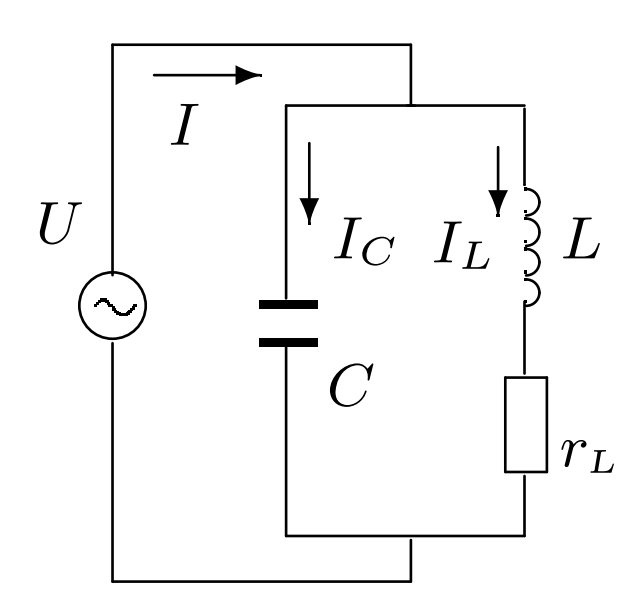
\includegraphics[width=0.5\textwidth]{Контур.png}
\end{center}
\caption{Параллельный контур}
\end{figure}
Обозначим через $r_{L}$ активное сопротивление катушки. Активным сопротивлением емкостной ветви контура обычно можно пренебречь. Рассмотрим установившиеся колебания в контуре, когда напряжение на нём меняется по гармоническому закону: $U=U_{0} \cos \Omega t$.

Введём обозначения для комплексных сопротивлений (импедансов)
индуктивной и емкостной ветвей контура:
$$Z_{L}=r_{L}+i \Omega L \quad \text { и } \quad Z_{C}=\frac{1}{i \Omega C}$$
Тогда полный импеданс контура может быть найден по правилу сложения параллельных сопротивлений:
\newpage
$$\frac{1}{Z}=\frac{1-\left(\Omega / \omega_{0}\right)^{2}+i r_{L} \Omega C}{r_{L}+i \Omega L}$$
где  — $\omega_{0}$ cобственная частота колебательного контура $\left(\omega_{0}^{2}=1 /(L C)\right)$.
Сопротивление контура равно модулю импеданса Z:
$$R_{\mathrm{pe3}}=|Z|_{\mathrm{pe3}}=\frac{L}{C r_{L}} \sqrt{1+\left(\frac{r_{L}}{\omega_{0} L}\right)^{2}}$$
В случае, когда активная часть импеданса индуктивной ветви много
меньше реактивной $\left(r_{L} \ll \omega_{0} L\right)$,
$$R_{\mathrm{pe} 3}=\frac{L}{C r_{L}}$$
Реактивные сопротивления обеих ветвей контура при резонансе равны,
поэтому, введя обозначение
\begin{equation}
\rho=\omega_{0} L=\frac{1}{\omega_{0} C}=\sqrt{\frac{L}{C}}
\end{equation}
можно записать
\begin{equation}R_{\mathrm{pe} 3}=\frac{\omega_{0}^{2} L^{2}}{r_{L}}=\frac{1}{r_{L} \omega_{0}^{2} C^{2}}=\frac{\rho^{2}}{r_{L}}\end{equation}
Учитывая, что добротность контура Q может быть выражена через
активное и реактивное сопротивления:
\begin{equation}Q=\frac{\omega_{0} L}{r_{L}}=\frac{1}{r_{L} \omega_{0} C}=\frac{\rho}{r_{L}}\end{equation}
получим ещё одну удобную для расчётов резонансного сопротивления
формулу:
\begin{equation}R_{\mathrm{pes}}=Q \cdot \rho\end{equation}
При резонансе значения токов в ветвях контура I L , рез , I C , рез и полного
тока в контуре I рез связаны с напряжением на контуре простыми соот-
ношениями:
\begin{equation}I_{L, \mathrm{pe} 3}=\frac{U}{\omega_{0} L}=\frac{U}{\rho}\end{equation}
\begin{equation}I_{C, \text { peз }}=U \omega_{0} C=\frac{U}{\rho}\end{equation}
\begin{equation}I_{\mathrm{pe3}}=\frac{U}{Q \rho}\end{equation}
Из этих выражений видно, что при резонансе токи в индуктивной и ем-
костной ветвях контура одинаковы и в Q раз больше тока в общей цепи:
\begin{equation}Q=\frac{I_{C, \text { peз }}}{I_{\text {pe3 }}}=\frac{I_{L, \text {pe3 }}}{I_{\text {pe3 }}}\end{equation}

\newpage
\subsection{Экспериментальная установка}
В работе изучается параллельный контур, одна из ветвей которого содержит индуктивность L, другая емкость C. Через $r_{L}$ обозначено активное сопротивление катушки, которое включает в себя как чисто омическое сопротивление витков катушки, так и сопротивление, связанное с потерями энергии при перемагничивании сердечника катушки. Активным сопротивлением емкостной ветви контура можнопренебречь, т. к. используемый в работе конденсатор обладает малыми потерями. 

Схема экспериментальной установки приведена на рис. 1. Напряжение от сети (220 В, 50 Гц) с помощью ЛАТРа через понижающий трансформатор Тр подается на параллельный контур, содержащий конденсатор (C = 120 мкФ) и катушку, индуктивность которой зависит от глубины погружения сердечника. Полный ток в цепи измеряется с помощью многопредельного амперметра A1; для измерения токов в L- и C-ветвях используются два одинаковых амперметра
A2 и A3; напряжение на контуре контролируется электронным вольтметром V. Последовательно с контуром включен резистор r - реостат с полным сопротивлением $\simeq$100 Ом. 

\begin{figure}[h!]
\begin{center}
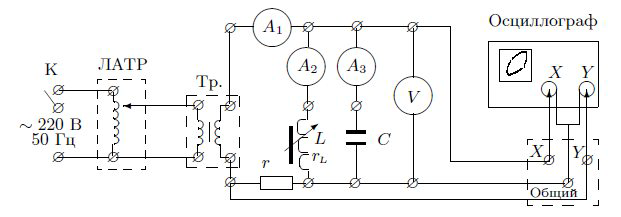
\includegraphics[width=0.9\textwidth]{Установка.png}
\end{center}
\caption{Cхема экспериментальной установки}
\end{figure}
Для наблюдения за сдвигом фаз между полным током и напряжением на контуре используется осциллограф. Сигнал, пропорциональный току,
снимается с резистора r и подается на вход Y осциллографа. На вход X
подается напряжение непосредственно с контура. При наличии сдвига
фаз между этими напряжениями на экране виден эллипс, а при нулевом
сдвиге фаз эллипс вырождается в прямую. 


\section{Практическая часть}
\subsection{Снятие показаний приборов}
Во время выполнения лабораторной работы были выполнены следующие действия:
\begin{itemize}
    \item Были сняты показания сил тока вцелом в цепи, на катушке индуктивности и на конденсаторе (на амперметрах A1, A2, A3 соответсвенно). Соответсвующие результаты занесены в таблицу 1. Последней строчкой указаны значения для резонансных токов (ток на катушке был измерен на более точном пределе измерений). У всех трех амперметров класс точности составлял 0,5 едениц (следовательно, погрешностью измерения тока можно считать половину цены деления прибора).
    \item Далее на месте была оценена добротность контура Q по формуле (8). 
    \item Были измеренны сопротивление витков катушки с помощью омметра. Также с помощью моста Е7-8 были измеренны сопротивление катушки $r_{L}$ и резонансное значение индуктивности L. Соответсветсвующие значения занесены в Таблицу 2.
\end{itemize}

\begin{table}[h!]
\begin{center}
\caption{Измерение токов}
\begin{tabular}{|c|c|c|c|}
\hline
L, mm & $I_{общ}$, A & $I_{L}$, A &  $I_{C}$, A \\ \hline
10    & 0,43        & 0,01        & 0,44        \\
15    & 0,34        & 0,10        & 0,44        \\
20    & 0,29        & 0,20        & 0,44        \\
25    & 0,26        & 0,22        & 0,44        \\
30    & 0,24        & 0,24        & 0,44        \\
35    & 0,21        & 0,27        & 0,44        \\
40    & 0,19        & 0,30        & 0,44        \\
45    & 0,16        & 0,33        & 0,44        \\
50    & 0,13        & 0,36        & 0,44        \\
55    & 0,11        & 0,38        & 0,44        \\
60    & 0,05        & 0,42        & 0,43        \\
65    & 0,05        & 0,45        & 0,44        \\
70    & 0,08        & 0,50        & 0,44        \\
75    & 0,13        & 0,54        & 0,44        \\
80    & 0,17        & 0,59        & 0,44        \\
85    & 0,22        & 0,65        & 0,44        \\
90    & 0,29        & 0,71        & 0,44        \\
95    & 0,36        & 0,78        & 0,44        \\
100   & 0,42        & 0,84        & 0,44        \\ \hline
62    & 0,06        & 0,43        & 0,43        \\ \hline
\end{tabular}
\end{center}
\end{table}

\begin{table}[h!]
\begin{center}
\caption{Характеристики цепи}
\begin{tabular}{|c|cc|}
\hline
f, кГц & \multicolumn{1}{c|}{L, мГн} & R, Ом \\ \hline
1      & 66,56                       & 38,2 \\
50     & 75.69                       & 3,53 \\ \hline
R, Ом      & \multicolumn{2}{c|}{4,05}       \\ \hline
Q      & \multicolumn{2}{c|}{7,48$\pm$0,24}          \\ \hline
\end{tabular}
\end{center}
\end{table}

\newpage
\subsection{Обработка результатов измерений}
На рисунке 3 проиллюстрирована зависимость токов через амперметры от глубины погружения сердечника катушки (за нуль принято положение в котором сердечник полностью опущен, полностью вынут он при х = 15см). Естественно что в момент резонанса  токи через конденсатор и катушку сравниваются, а общий ток в цепи достигает своего минимума. Резонансные значения на графике отмечены пустым ромбом.

 \begin{figure}[h!]
\begin{center}
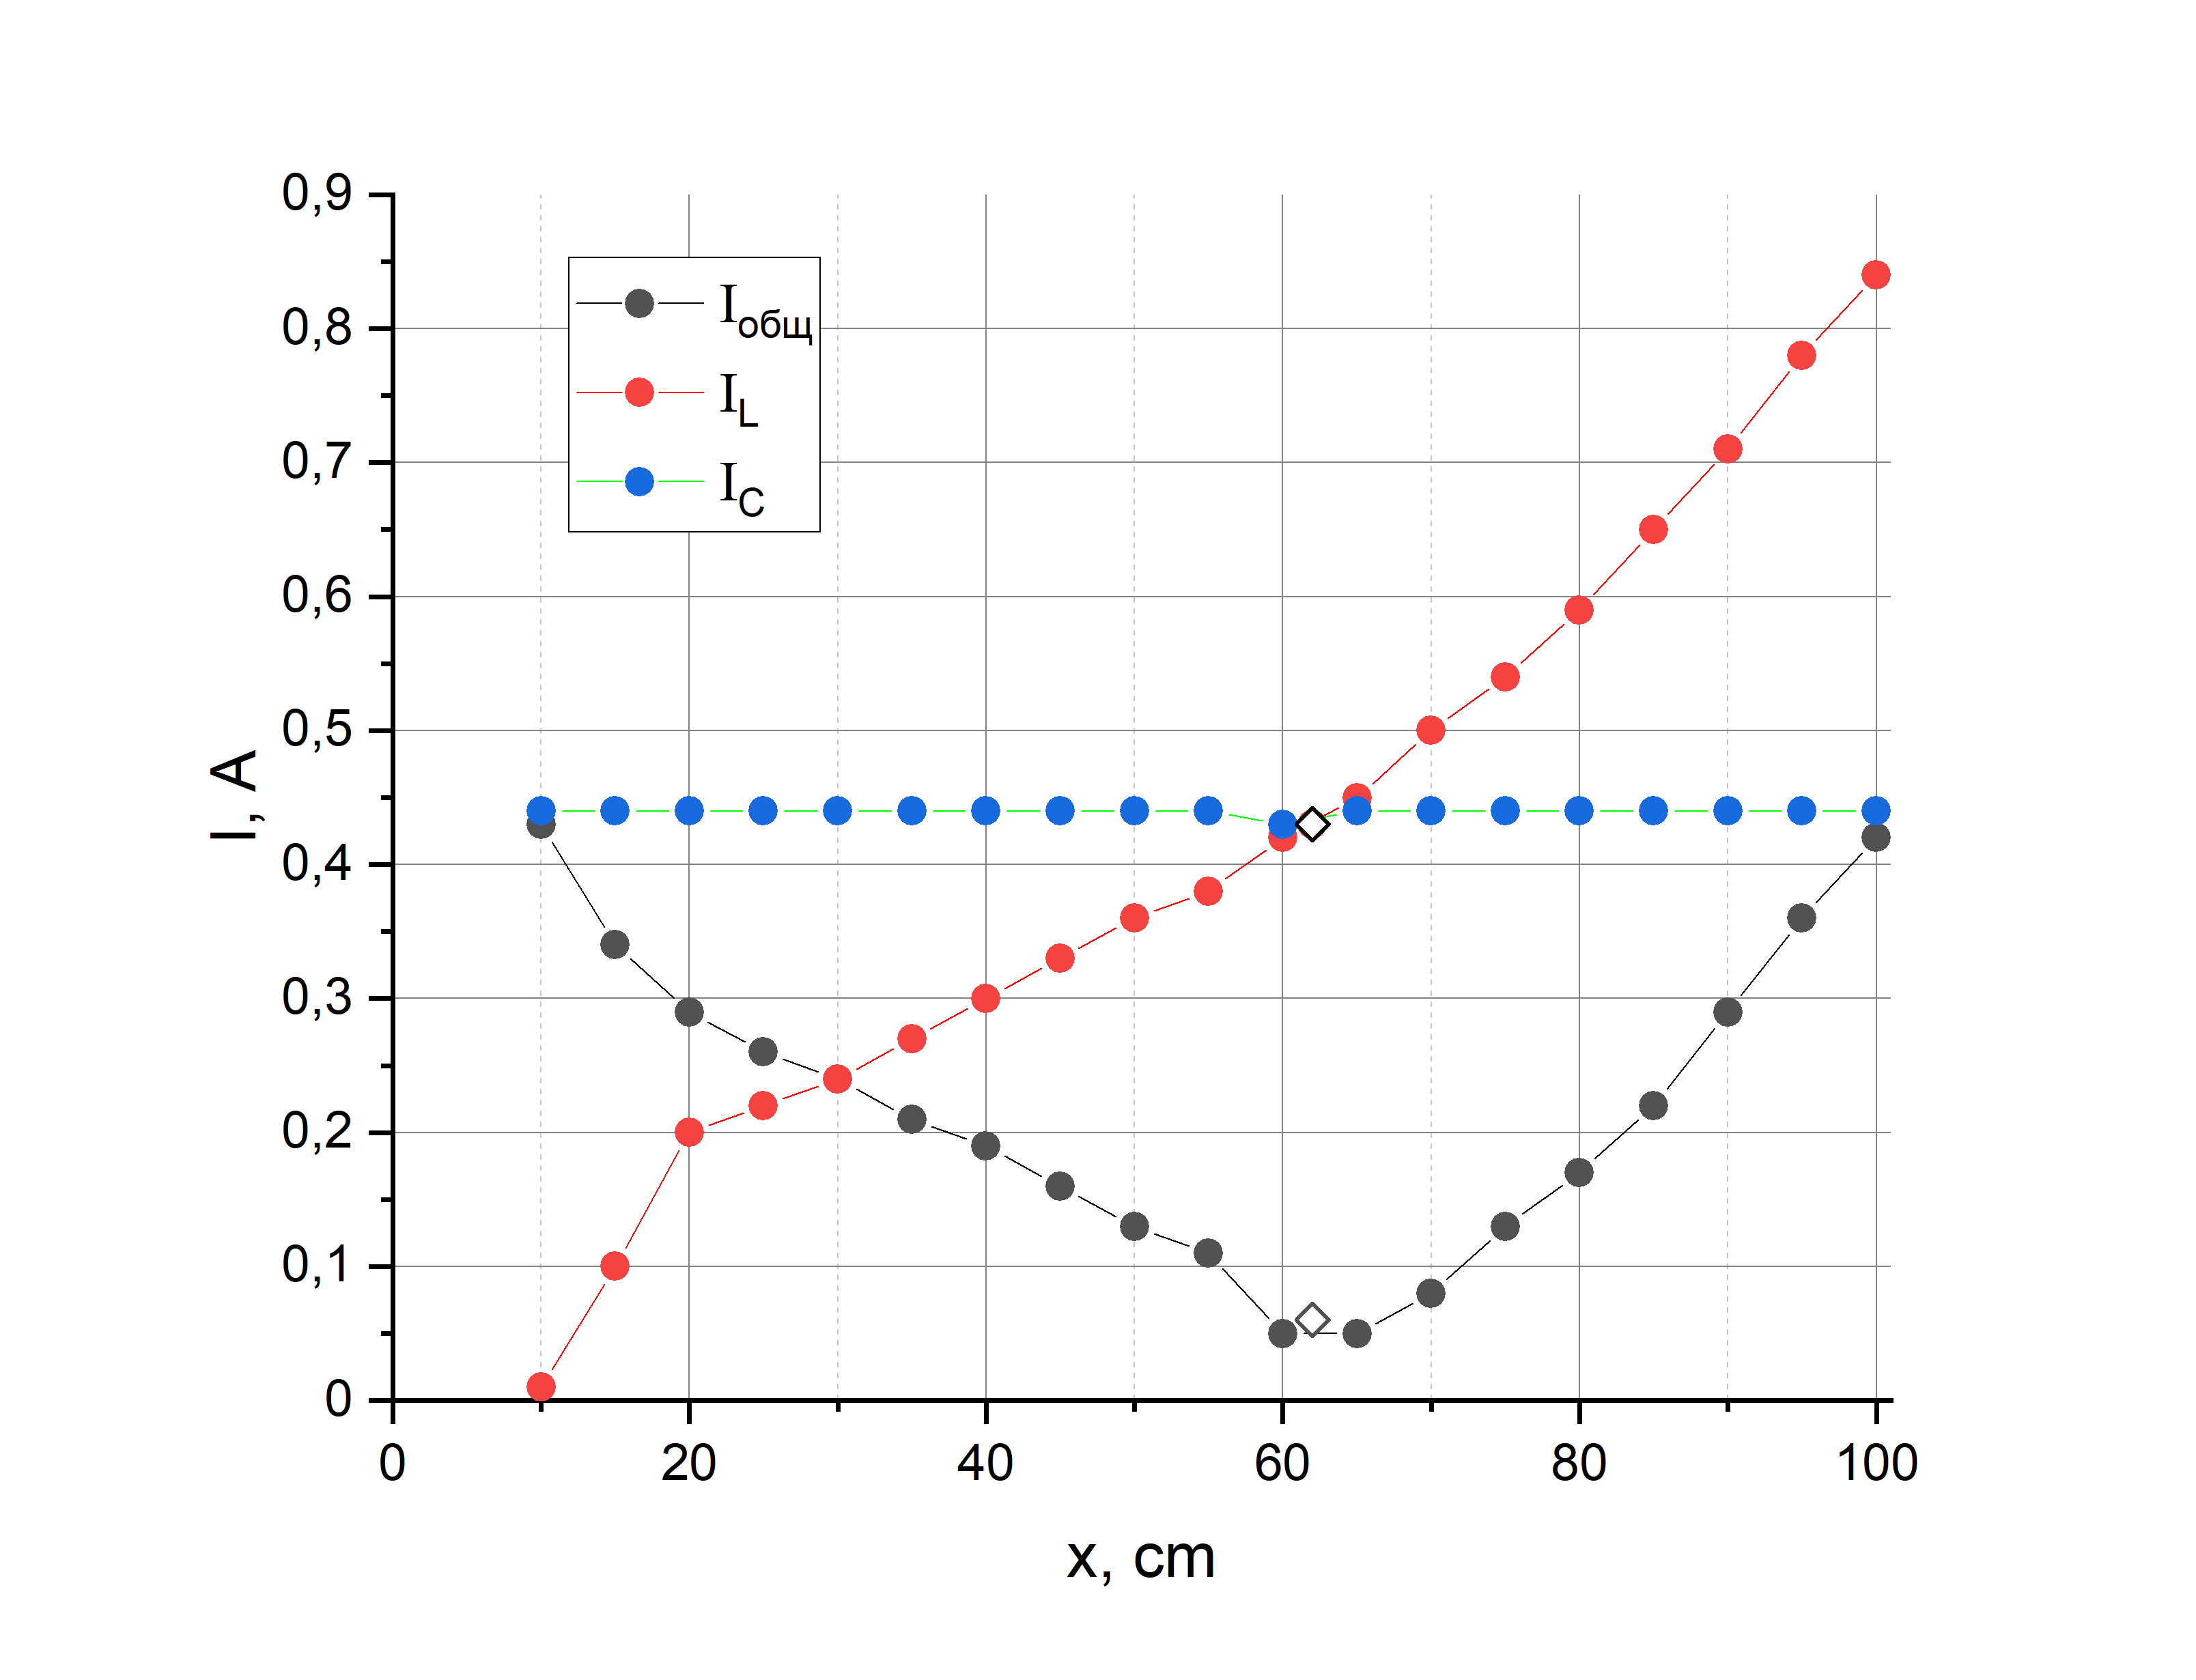
\includegraphics[width=0.7\textwidth]{Graph2.png}
\end{center}
\caption{Зависимость токов от глубины погружения сердечника катушки}
\end{figure}
\begin{enumerate}
    \item Зная добротность цепи можно по формулам (4) и (7) расчитать:
 \begin{displaymath}R_{\mathrm{pe3}}=\frac{U}{I_{\mathrm{pe3}}}= 174 \pm 10 \, \Omega\end{displaymath}
    \iteml Из формулы (3): \begin{displaymath} L_{p e3}=\frac{1}{4 \pi^{2} \nu^{2}_{0} C}= 84,4 \, \text{мГн}, \;  r_{L}=\frac{1}{2 \pi \nu_{0} \mathrm{QC}} = 3,55 \pm 0,11 \, \Omega \end{displaymath}
    \item Резонансная индуктивность из (5): \begin{displaymath}L_{ \mathrm{pe} 3}=\frac{U}{\omega_{0}I_{L, \mathrm{pe} 3}} =74 \pm 5 \, \text{мГн}\end{displaymath}
    \item Построеная в масштабе векторная диаграма для токов и напряжений приведена на рисунках 4 и 5. Из нее мы можем рассчитать значения сопротивления индуктивности катушки, значения занесены в таблицу 3.
    \begin{figure}[h]
\begin{center}
\begin{minipage}[h]{0.49\linewidth}
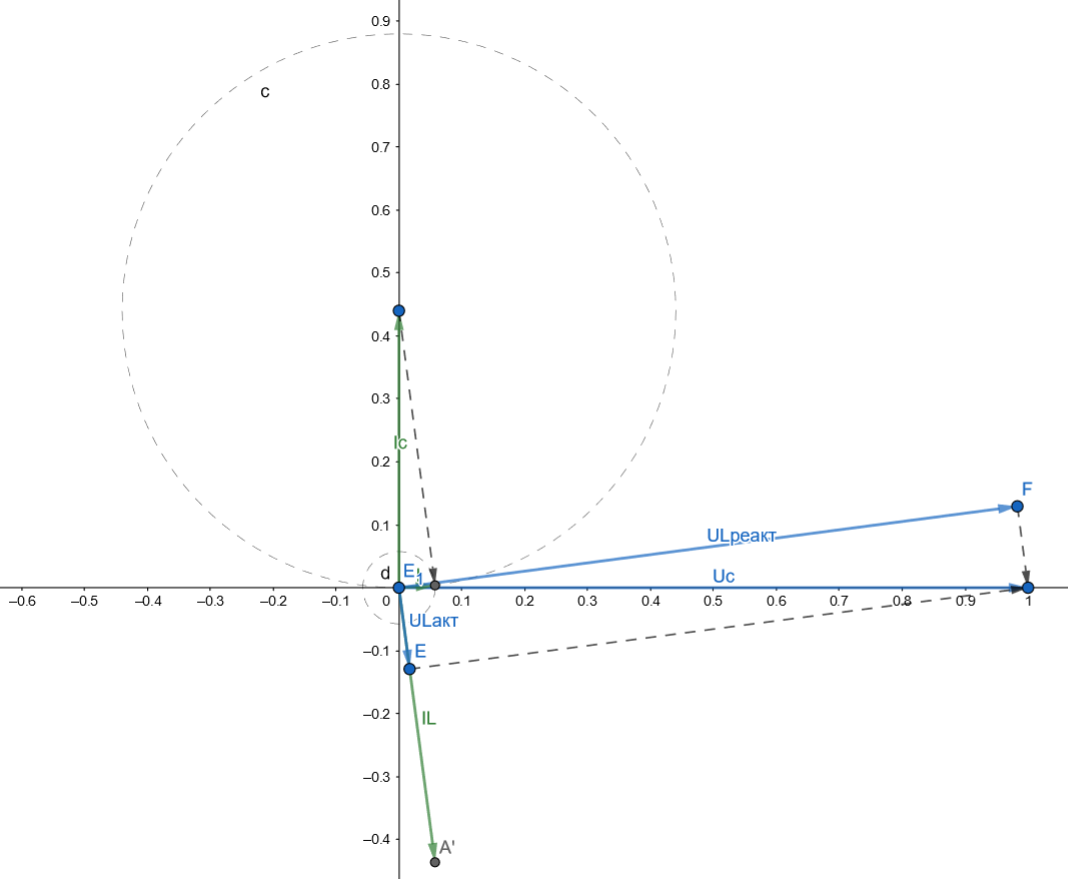
\includegraphics[width=1\linewidth]{Большой.png}
\caption{Общий план} %% подпись к рисунку
\label{ris:experimoriginal} %% метка рисунка для ссылки на него
\end{minipage}
\hfill
\begin{minipage}[h]{0.49\linewidth}
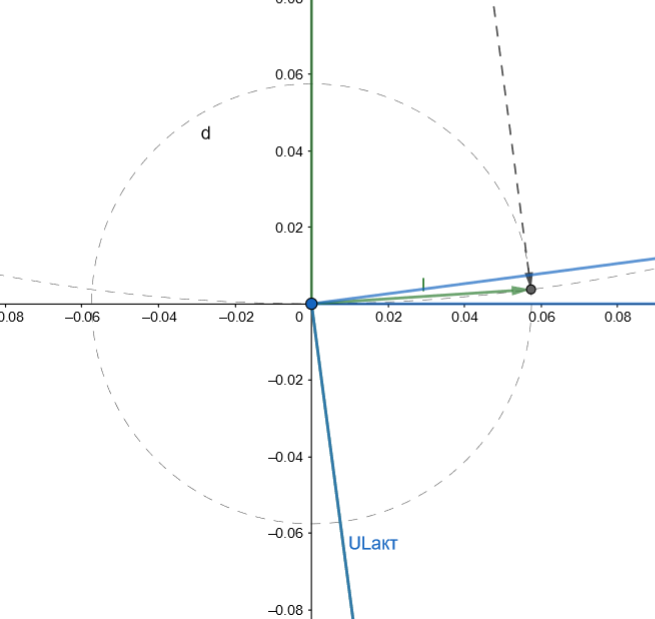
\includegraphics[width=0.88\linewidth]{Малый.png}
\caption{Приближенный план}
\label{ris:experimcoded}
\end{minipage}
\end{center}
\end{figure}
\begin{table}[!h]
\begin{center}
\caption{Сравнение методов}
\begin{tabular}{|c|c|c|c|c|c|}
\hline
   & Омметр & Мост Е7-8 & $f(U_{res}, I_{L, res})$ & f(Q)         & Вект. диаг. \\ \hline
$r_{L}, \Omega$ & 4,05   & 3,53      & --             & 3,55 $\pm$ 0,11 & 3,02        \\ \hline
L, мГн  & --     & 75,69     & 74 $\pm$ 5        & 84,4         & 73,2        \\ \hline
\end{tabular}
\end{center}
\end{table}

\end{enumerate}
\newpage
 \section{Выводы}
 Как видно из таблицы 3, в эксперименте имелась возможность расчитать сопротивление и индуктивность катушки различными способами. Трудно поддается объяснению тот факт, что сопротивление измеренное с помощью омметра меньше сопротивления измеренного на мосту. Теоретически наиболее точное значение для L можно было получить из формулы (2), так как оно было выведено лишь из того факта, что реактивные сопротивления обоих элементов в резонансе равны. Однако как раз оно наиболее отлично от остальных, что, возможно(?), объясняется падением емкости конденсатора со временем. расчет же через резонасные значения напряжения и тока и через векторные диаграмы для индуктивности дал значения близкие к измеренным на мосту
\end{document}

